% -*-coding: utf-8 -*-

\BiAppChapter{相关内容补充}{}

\BiSection{硬件交互}{}\label{app-interaction}
手机图像实时传入到模型中的流程如下:手机通过USB连接到主机,
通过Scrcpy\footnote{\url{https://github.com/Genymobile/scrcpy}\hfill}将视频流信息通过Linux内核中V4L2传入到虚拟设备中,
再通过OpenCV-Python\footnote{\url{https://github.com/opencv/opencv-python}}从虚拟设备中获取到视频流数据,
流程图如图~\ref{fig-framework}~所示。

\BiSection{动态采样概率分布}{}\label{app-dynamic-distrib}
动态概率分布用于切片的中心点位选取,可以将生成的单位形成团簇,产生更多重叠部分,能有效提高识别数据的多样性,
具体实现过程如下,设当前待选取点位为离散的$W\times H$矩阵,切片的待选二维离散分布为$D:\{1,2,\cdots,W\}\times \{1,2,\cdots,H\}\to \mathbb{R}$,
动态修改范围为$S=3$,
令$(i,j)\sim D$,则修改$D$中以$(i,j)$为中心附近大小为$S\times S$的分布:
\begin{equation}\label{eq-dynamic-distrib}
	\begin{bmatrix}
		d_{i-1,j-1}&d_{i-1,j}&d_{i-1,j+1}\\
		d_{i,j-1}&d_{ij}&d_{i,j+1}\\
		d_{i+1,j-1}&d_{i+1,j}&d_{i+1,j+1}\\
	\end{bmatrix}\to 
	\frac{1}{f(d_{ij})}\begin{bmatrix}
		d_{i-1,j-1}&d_{i-1,j}&d_{i-1,j+1}\\
		d_{i,j-1}&\frac{f(d_{ij})}{2}d_{ij}&d_{i,j+1}\\
		d_{i+1,j-1}&d_{i+1,j}&d_{i+1,j+1}\\
	\end{bmatrix}
\end{equation}
其中$f(d_{ij}) = \frac{d_{ij}}{2\sum_{u,v=1}^{S}[d_{i+u,j+v}\neq 0]}$。做法是使中心概率下降$d_{ij}/2$,
并将周围的非零概率点位平均分配$d_{ij}/2$。

% \BiSection{生成式数据集实例}{}
% 通过调整不同的单位生成数量(20、40)、切片生成类型(小型、大型),最大覆盖阈值$\alpha$($0.5, 0.8$),可以得到如图~\ref{fig-app-generation}~所示的生成结果。
% \begin{figure}
% \centering
% \subfigure[单位生成数量20,小型切片类型,$\alpha=0.5$]{
\includegraphics[width=0.32\textwidth]{generation/nu20,small,0.5.jpg}}
% \subfigure[单位生成数量20,大型切片类型,$\alpha=0.5$]{
\includegraphics[width=0.32\textwidth]{generation/nu20,big,0.5.jpg}}
% \subfigure[单位生成数量20,大型切片类型,$\alpha=0.8$]{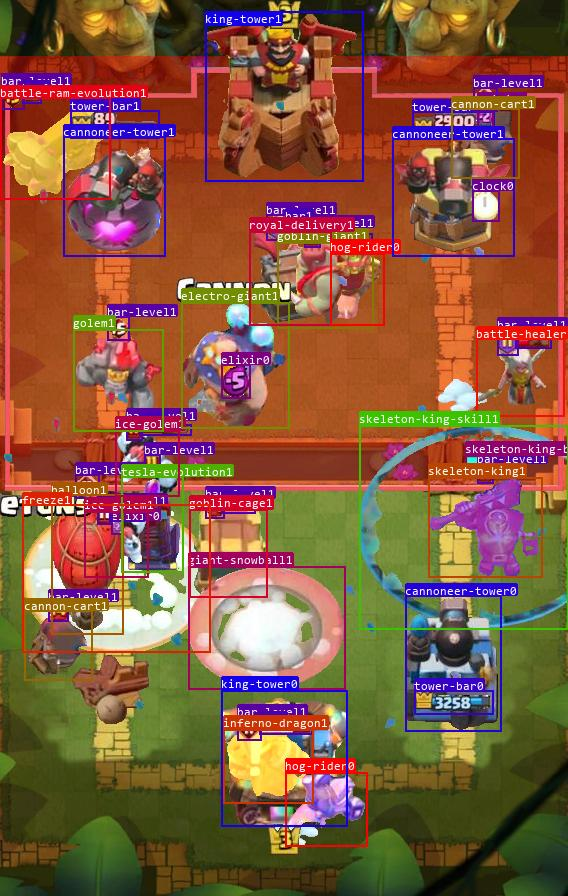
\includegraphics[width=0.32\textwidth]{generation/nu20,big,0.8.jpg}}
% \subfigure[单位生成数量40,小型切片类型,$\alpha=0.5$]{
\includegraphics[width=0.32\textwidth]{generation/nu40,small,0.5.jpg}}
% \subfigure[单位生成数量40,大型切片类型,$\alpha=0.5$]{
\includegraphics[width=0.32\textwidth]{generation/nu40,big,0.5.jpg}}
% \subfigure[单位生成数量40,大型切片类型,$\alpha=0.8$]{
\includegraphics[width=0.32\textwidth]{generation/nu40,big,0.8.jpg}}
% %\vspace{4ex}
% \caption{生成式数据集实例}\label{fig-app-generation}
% \end{figure}

\BiSection{数据增强}{}
\begin{table}[!h]
	\renewcommand{\arraystretch}{1.2}
	\centering\wuhao
	\caption{数据增强参数范围} \label{table-app-aug} \vspace{2mm}
	\begin{tabularx}{\textwidth} { 
   >{\centering\arraybackslash}X 
   >{\centering\arraybackslash}X 
   >{\centering\arraybackslash}X }
	\toprule[1.5pt]
  数据增强类型&参数变换范围&单位\\
	\midrule[1pt]
	HSV增强&$\pm(0.015,0.7,0.4)$&比例系数\\
	图像旋转&$(-5,5)$&度\\
	横纵向随机平移&$(-0.05,0.05)$&比例系数\\
	图像缩放&$(-0.2,0.2)$&比例系数\\
	图像左右反转&$0.5$&概率大小\\
	\bottomrule[1.5pt]
	\end{tabularx}
\end{table}

\newpage
\BiSection{模型测试卡组}{}\label{app-sec-desk}
\begin{table}[!h]
	\renewcommand{\arraystretch}{1.2}
	\centering\wuhao
	\caption{我方卡组(平均圣水花费2.6)}\vspace{2mm}
	\begin{tabularx}{\textwidth} { 
   >{\centering\arraybackslash}X 
   >{\centering\arraybackslash}X 
   >{\centering\arraybackslash}X 
   >{\centering\arraybackslash}X }
	\toprule[1.5pt]
	卡牌名称&类型&攻击目标&圣水花费\\
	\midrule[1pt]
	骷髅兵&部队&地面&1\\
	冰雪精灵&部队&地面和空中&1\\
	滚木&法术&地面&2\\
	戈仑冰人&部队&建筑&2\\
	加农炮&建筑&地面&3\\
	火枪手&部队&地面和空中&4\\
	野猪骑士&部队&建筑&4\\
	火球&法术&地面和空中&4\\
	\bottomrule[1.5pt]
	\end{tabularx}
\end{table}

\begin{table}[!h]
	\renewcommand{\arraystretch}{1.2}
	\centering\wuhao
	\caption{8000分内置AI敌方卡组(平均圣水花费4.6)}\vspace{2mm}
	\begin{tabularx}{\textwidth} { 
   >{\centering\arraybackslash}X 
   >{\centering\arraybackslash}X 
   >{\centering\arraybackslash}X 
   >{\centering\arraybackslash}X }
	\toprule[1.5pt]
	卡牌名称&类型&攻击目标&圣水花费\\
	\midrule[1pt]
	野蛮人滚筒&法术&地面&2\\
	飓风法术&法术&地面和空中&3\\
	狂暴樵夫&部队&地面&4\\
	骷髅飞龙&部队&地面和空中&4\\
	野蛮人&部队&地面&5\\
	雷电飞龙&部队&地面和空中&5\\
	圣水收集器&建筑&无&6\\
	戈仑石人&部队&建筑&8\\
	\bottomrule[1.5pt]
	\end{tabularx}
\end{table}
注:测试时间为2024年5月,第59赛季。

